\section{Ausblick - Autonomes Fahren} \label{sec:ausblick}

Wie bereits bei der Analyse der Ergebnisse festgestellt wurde, ist das Erkennen von Hindernissen mit anschließendem Ausweichen nur ein erster kleiner Schritt auf dem Weg zum autonomen Fahren. Und selbst diese einfach anmutende Aufgabe scheint nie Perfekt umsetzbar zu sein. Das Ziel wird es in Zukunft werden, über mehr Trainingsdaten, komplexere neuronale Netze und schnellere Hardware das Fahren sicherer zu gestalten.\\
Da die Kollisionsvermeidung am Ende jedoch leichter umzusetzen war, als Anfangs erwartet, findet sich in diesem Ausblick auch eine weitere Live-Demo wieder. Konkret konnte zusätzlich die Fähigkeit umgesetzt werden einer Straße \bzw vielmehr den Straßenmarkierungen zu folgen. Dazu wurden wie auch schon in \autoref{sec:durchführung} drei Phasen durchlaufen:

\begin{enumerate}
    \item Datensammlung
    \item Trainieren des CNN
    \item Einsatz des trainierten Modells
\end{enumerate}

Der wesentliche Unterschied im Vergleich zur Umsetzung der Fähigkeit zur Kollisionsvermeidung bestand dabei vor allem in der Aufnahme und Klassifizierung der Daten. Der Jetbot wurde dafür auf einer Klemmbaustein-Straße an verschiedenen Positionen platziert. An den Positionen wurden erneut Bilder aufgenommen, diesmal jedoch mit einer zusätzlichen grünen Markierung, welche dem neuronalen Netz zeigen soll, wohin der Roboter sich bewegen sollte, wenn er sich in einer vergleichbaren Position befindet. \\
Auch hier war es möglich den Jetbot auf einer kleinen Demo-Strecke im Kreis fahren zu lassen.

\begin{figure}[H]
    \centering
    \fbox{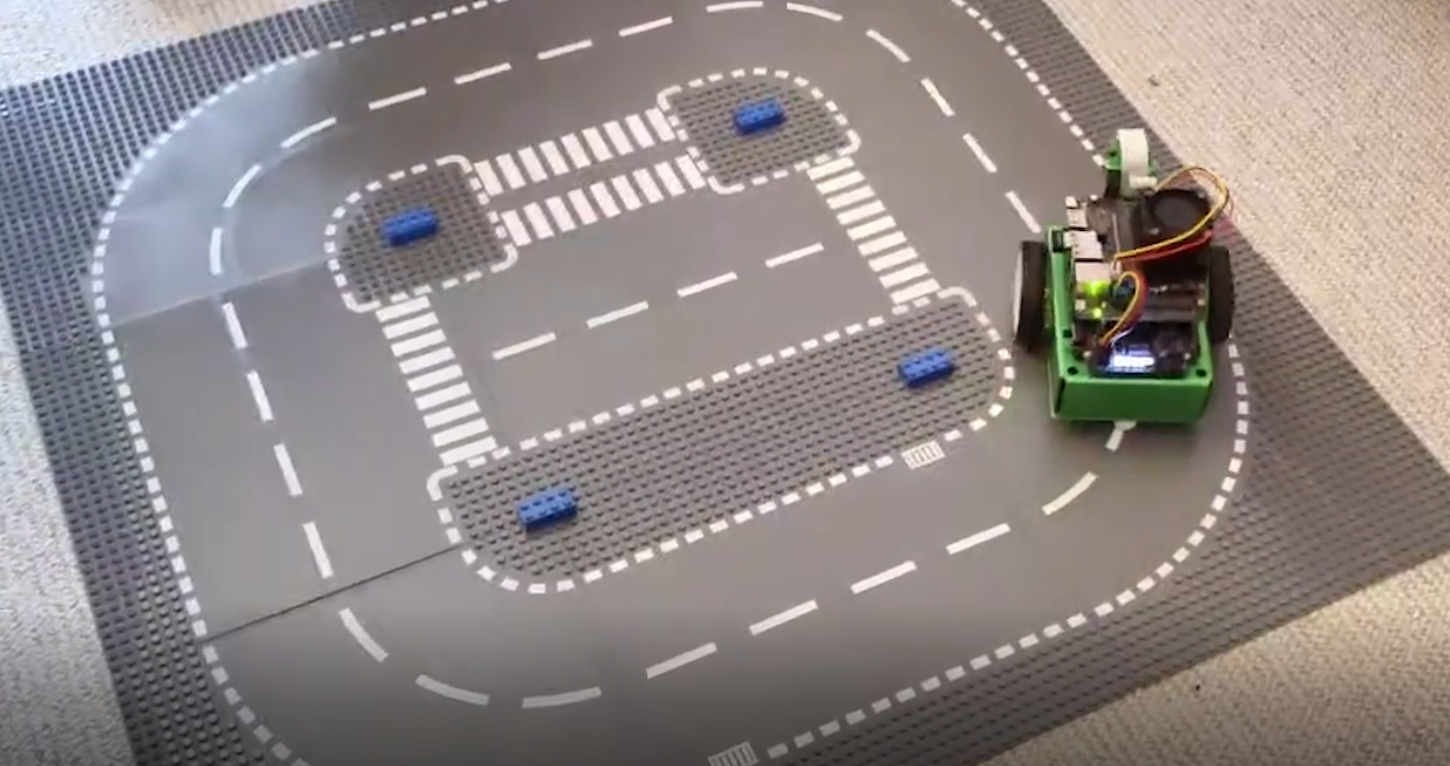
\includegraphics[width=0.65\textwidth]{Bilder/roadfollowing.png}}
    \caption[Folgen von Straßenmarkierungen]{Testversuch zum autonomen Fahren unter Vorgabe von Straßenmarkierungen}
    \label{fig:Bild6.1}
\end{figure}

Codebeispiele in Form von Jupyter Notebooks finden sich auch hierfür im Anhang wieder.